\chapter{Design and Implementation of Proposed Work}
This chapter will show the architectural, Algorithm, and class diagrams of the application,In this chapter also, the implementation of the proposed work will be explained which shows how genetic algorithm approach can be applied to cryptanalysis task, which does not have clear solution except for exhaustive search: breaking the Transposition and substitution cipher.
In this work, cryptanalysis used GA for searching the decryption key or getting maximum information about the decryption key. The Genetic Algorithm is a search and optimization techniques based On Darwin is the Principle of Natural Selection,
In Figure \ref{Cryptanalysis_flow} Flowchart of proposed method of cryptanalysis.
\begin{figure}[ht]
	\centering
	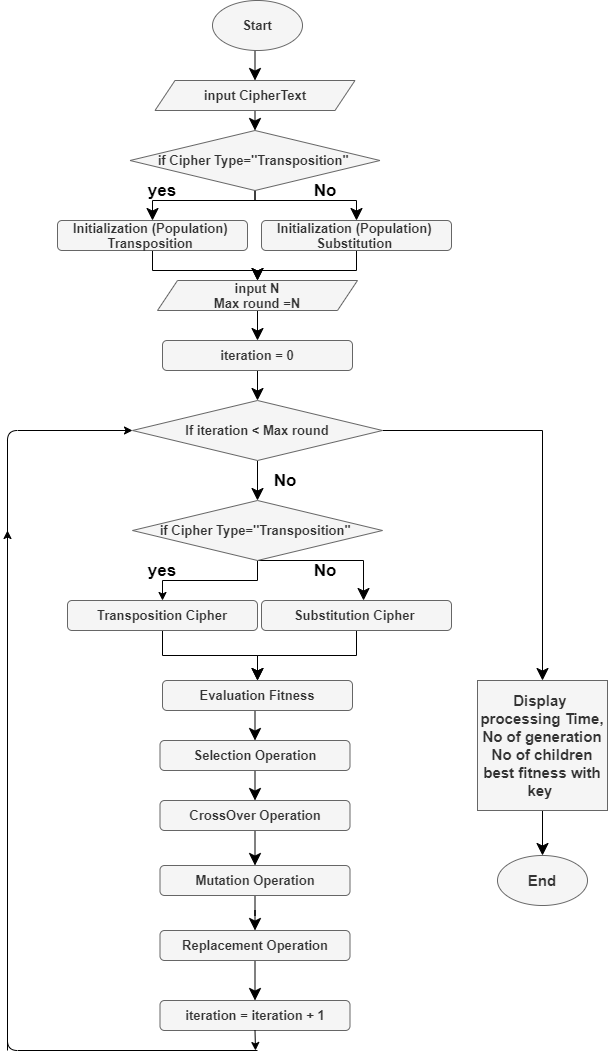
\includegraphics[width=.8\textwidth]{imagenes/FlowChartOfCry.png}
    \caption{Flowchart Of Proposed Method Of Cryptanalysis}
    \label{Cryptanalysis_flow}
\end{figure}
\section{Design of the work}
As we saw in Figure \ref{Cryptanalysis_flow} that we have nine main parts in the project Consequently, project design will content 9 dependency classes, first of them will be the main class which controls other classes as shown in Figure \ref{classes} and explains inheritance relationship between classes, In this section, we will explain the stages of project development as follows:
\newpage
\clearpage
\begin{figure}[h]
	\centering
	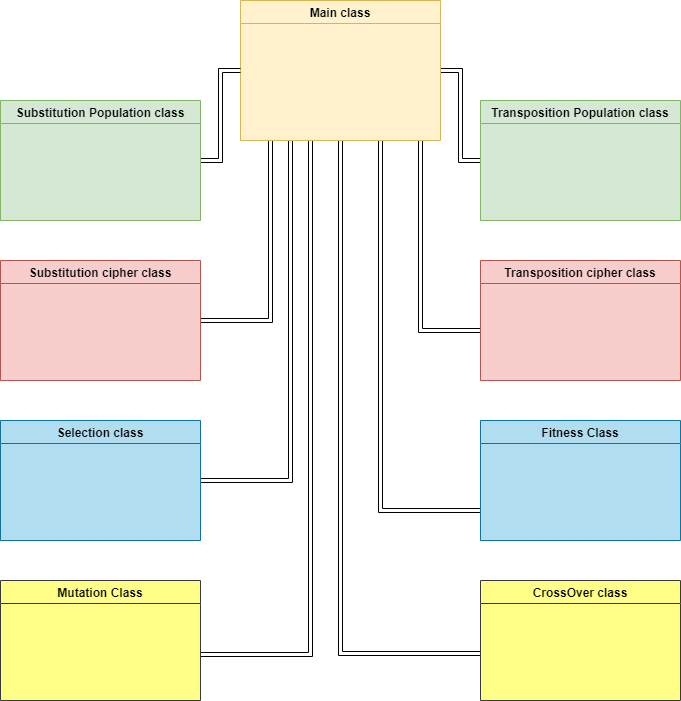
\includegraphics[width=.8\textwidth]{imagenes/classes.png}
    \caption{Inheritance relationship between the classes}
    \label{classes}
\end{figure}
\subsection{Population}
This part of the project is divided into two parts, depending on the cipher type:
\subsubsection{Transposition cipher population:}
In the initialization stage, generate a pool of random keys (size population), when the length of the key is N digits (chromosome size) and the pool size is M keys(size population). Also, The key condition is random and non-repetitive in each key. 
\subsubsection{Substitution  cipher population:}
on the other side, generate a pool of keys (size population), when the length of the key is 26 characters which equals the number of English letters (chromosome size) and the pool size is M keys(size population). Also, The key condition is random and non-repetitive in each key. These keys are changeable by the other stages of GA and the better one used in derivation the plaintext.
\subsection{Breaking Cipher}
in this stage, we will try to break the ciphertext using the keys which we got from the previous stage.
\subsubsection{Transposition Cipher:}
The transposition cipher is rearranged (change position only) the characters in the message but not change the characters. Transposition cipher has a pool of keys and ciphertext that rearranged the ciphertext for M times depending on the pool of keys. The output of transposition cipher saved in an array of M locations we can be called \textit{plaintext array}.
\subsubsection{Substitution Cipher:}
The substitution cipher replaces every instance of a particular letter in the ciphertext with a different letter from the cipher key, Thus a substitution cipher key can be defined as the set of one-to-one mappings relating every letter in the ciphertext alphabet with the corresponding letter in plaintext alphabet, so The Substitution cipher is changing the characters in the message but not change the characters positions, substitution cipher has a pool of keys and ciphertext that changed the ciphertext for M times depending on the pool of keys. The output of substitution cipher saved in an array of M locations which we can be called \textit{plaintext array}.
\subsection{Evaluation Fitness}
Fitness is evaluated based on the unigrams(one letter) frequencies, the bigrams (sequence of two letters) frequencies in the decrypted ciphertext, and Trigrams (sequence of three letters) frequencies in the decrypted ciphertext. the tables below illustrated the most popular bigrams and Trigrams in the English language. Trigrams and diagrams are computationally expensive the fitness calculation. The idea of the fitness function is the following \cite{Text_fitness}:
\begin{enumerate}
    \item{We take large text corpus and calculate the occurrences of unigrams, bigrams, and trigrams \begin{align*}& C^u_i, C^b_{ij}, C^t_{ijk} \end{align*}}
    \item{Then we sum all counters to get total sum of unigrams, bigrams and trigrams, \begin{align*}& S_u, S_b, S_t\end{align*}}
    \item{Then we calculate reference frequencies of each unigram, bigram and trigram,\begin{align*}& R^u_i = \frac{C^u_i}{S_u},R^b_{ij} = \frac{C^b_{ij}}{S_b},R^b_{ijk} =\frac{C^t_{ijk}}{S_t}\end{align*} }
    \item{Then, using the same method, we calculate the frequencies within the target text to obtain partial frequencies of each unigram, bigram and trigram, \begin{align*}& P^u_i, P^b_{ij}, P^t_{ijk} \end{align*} }.
    \item{Then we calculate the fitness score using the following formula:
    \begin{align*}
        F_i=\alpha \sum(R^u_i-P^u_i)+\beta \sum(R^b_{ij}-P^b_{ij})+\gamma \sum(R^t_{ijk}-P^t_{ijk})
    \end{align*}
where alpha, betha and gamma are the weights we assign to the importance of unigrams, bigrams and trigrams respectively. This implementation uses 1/6, 1/3 and 1/2, assigning most of the weight to trigrams}
\end{enumerate}
frequencies of unigrams, bigrams and trigrams are shown in the tables \ref{UI}\ref{TIBI1}\ref{TIBI2} respectively.
\begin{table}[h!]
    \centering
    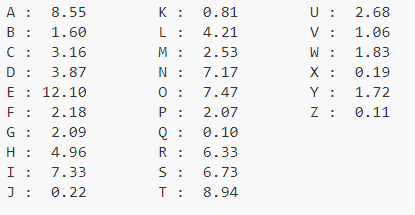
\includegraphics[width=0.8\textwidth]{imagenes/UI.png}\\
    \caption{English single letter frequencies}
    \label{UI}
\end{table}
\begin{table}[h!]
    \centering
    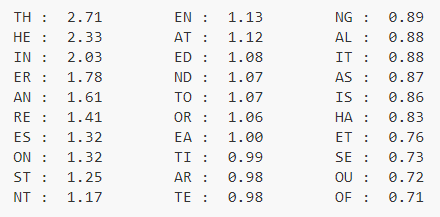
\includegraphics[width=0.8\textwidth]{imagenes/TIBI1.png}\\
    \caption{ The bigram frequencies}
    \label{TIBI1}
\end{table}
    \begin{table}[h!]
    \centering
    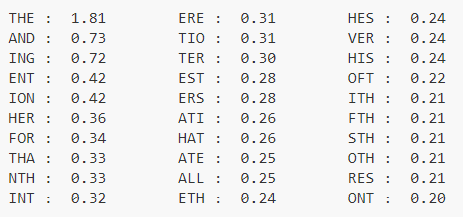
\includegraphics[width=0.8\textwidth]{imagenes/TIBI2.png}\\
    \caption{The trigram frequencies}
\label{TIBI2}
\end{table}
\newpage
\subsection{Selection}
In this operation, selection (choosing) the best keys only. The best key which has a high value of fitness. In the proposed work select only M/2 keys that have high fitness. To perform the selection operation needed a sorting function to sort pool of keys from high fitness to low fitness.

Fitness Proportionate Selection is one of the most popular ways of parent selection. In this stage, every individual can become a parent with a probability that is proportional to its fitness. Therefore, fitter individuals have a higher chance of mating and propagating their features to the next generation. Therefore, such a selection strategy applies a selection pressure to the more fit individuals in the population, evolving better individuals over time.
\subsection{CrossOver}
from the selection steps we got the best half of the population after calculating the fitness values, in this section, we generate a new population from the parents to get the children which represent the next generation, we can generate 2 children by using ( one point, two-point or uniform crossover operators )for each pair parents, but that gives us just half number of the original population, so can we use two methods to generate a new population, for instance, every 2 parents give us 4 children, the first 2 children are generated using one-point crossover operator and the other children are generated using uniform crossover operator,
in another way to keep the same number of population, we can keep the parents to the next generation, Through experiences, we can discuss which one is best to use, for that we applied all of them in this part to make the application more flexible.
\subsection{Mutation}
In this operation, applying the mutation operation for the new population. To perform the mutation operation, two random numbers generated such as R1, and R2 representing two positions in each key then swap between the value of the position R1 and the value of the position R2. Repeat this operation for all keys in the "new population" pool.
\subsection{Display The Results}
In this operation, display the plaintext (clear text is unencrypted information) for storage or transmission after decrypting the ciphertext. Also, display  the fitness values, the number of geneerations and te number individuals.
\section{Implementation of the proposed work}
\subsection{Population Steps}
the first class to start is Population.java in this class we created the Population which represents a set of chromosomes and each chromosome has the same length so, Population class has one constructor and many methods that follow:
\textsf{Population Constructor:} this constructor has two parameters:
\begin{itemize}
    \item{\textsf{NoOFkeys:} No. of chromosomes}
    \item{\textsf{lengthOFkey:} length of the chromosome.}
\end{itemize} 
under this Constructor, we can call all of the methods to create our population and show it. The first method is \textit{IFKEYEXIST} this method will generate a set of numbers between 1 and length of chromosome without repeat numbers (non-repetitive) and randomly, Method \textit{check} is created to ensure there are no duplicated numbers and check method has two parameters the first is an array of numbers are saved before and the second is a new number which will save in the same array,
and return true or false (if this new number exist in the array of the chromosome will return false in another case will return true and save it) after getting more then 2 chromosomes we have to check if there are duplicate chromosomes this step done with this method which called \textit{checkrow} which receive all of the chromosomes that saved before and new chromosome after that will compare between them to find if there are duplicated between these chromosomes, then will return false if there are no chromosomes duplicated and save it, if not, it will repeat the step of creating new chromosome.
\textsf{Note*}
this population will use to breaking Transposition cipher when we wanted to create a population to breaking Substitution Cipher we have created a new population class with some changes as follow:
the constructor of the substitution population class has just one parameter which is a no. of keys(No. of chromosomes) then we generated 26 characters from A to z randomly without repeating, so the length of the chromosome will be 26 characters are sorted randomly and non-repetitive.


\subsection{Trnsposition Steps}
The second step is Transposition Cipher, in this class Transposition.java we will try to get the origin text by using exchange the positions of characters as I explained in the section of Transposition Cipher, so if we have 16 keys, we can get 16 texts that may be the plaintext, in this class, we have 4 methods and one constructor, this class has:
\begin{itemize}
    \item{\textsf{Transposition constructor:} this Constructor has two parameters the array of keys which we got from Population class and ciphertext, then we will call methods that follow:}
\begin{enumerate}
    \item{\textsf{check if lenNotDivid} We created this method to enforce the message length, adding an "X" to the end of the message, making the message proportional to the key length.}
    \item{\textsf{change position} this method splits the ciphertext as blocks, the length of each block equals the length of the key, then call the SortbyKey method with sending one of the keys and one of the blocks to exchange the characters positions in each block.}
    \item{\textsf{SortByKey} this method receives one of the keys and one block of ciphertext and then exchanges the positions of all characters in that block depending on that key.}
    \item{\textsf{Print} this method called in the Transposition constructor to print the array of PlainText after doing the Transposition.}
\end{enumerate}
\end{itemize}


\subsection{Substitution Steps}
Substitution.java we will try to get the origin text by using change the  characters as I explained in the section of Substitution Cipher, so if we have 16 keys, we can get 16 texts that may be the plaintext, in this class, we created a constructor, under this constructor we created  new array to save texts after doing Substitution process, then we called a substitution method which responsible to change ciphertext to another text depending on the keys,
under this method, we convert each character in ciphertext to ASCII code then apply an equation to get the index of this character from the keys array,  \textit{an instance:}
\begin{tcolorbox}[breakable,notitle,boxrule=0pt,colback=blue!20,colframe=blue!20]
    {key= K H N E I B F G M D L U J V S P C Y Q R T X Z O  W  A\\
    ciphertex=HTSCRJ\\
    then we can get every character ASCII\\
    ASCII(H)=73\\
    ASCII(H)= ASCII(H)-65 so, ASCII(H)=8,\\
    GetIndex(8) form Key array\\
    H=G\\
    repeat this process to get every characters\\
    so, PlainText= GUOQTM
     }
    \end{tcolorbox}


\subsection{Fitness Evaluation steps}
with this step we created a new class, we called it, Fitness.java, this class contents on one constructor and set of methods to calculate fitness step by step, The first thing we did it is creating 6 arrays that follow:
\begin{itemize}
    \item{\textsf{monogram:} to save the unigram score(weight)}
    \item{\textsf{Twochar:}to save the bigram frequencies.}
    \item{\textsf{TwoCharVale} to save the bigram score(weight).}
    \item{\textsf{Threechar:}to save the trigram frequencies.}
    \item{\textsf{ThreeCharVale} to save the trigram score(weight).}
\end{itemize}
now, we are going to start with Fitness constructor which receives the Array of PlainTexts which we got  from Transipostion step and Array of keys(chromosomes), under this constructor, we initialized a set of arrays to save the summation of bigram frequencies of each PlainText, trigram frequencies summation, and unigram, and we created another array to save the final value of fitness for each PlainText, then we called methods to start calculating which follow:
\begin{itemize}
    \item{\textsf{FitnessMethod:} to save the unigram score(weight)}
    \item{\textsf{fitnessequation:}under this method, we will calculate the final value of fitness for each PlainText by using the equation and save it in Fitness array.}
\end{itemize}


\subsection{Selection Steps}
After getting fitness array for each PlainText from the previous step, it is time to select the best parents to generate a new population from those parents, let us firstly sort the fitness array descending then select the best half of that array by using high fitness, in the Selection.java class, we have one selection contracture which receives three parameters (the keys Array(chromosomes), PlainTexts Array, fitness Array ), under this contractor the first thing we have done it is initializing a set of arrays,
\begin{itemize}
    \item{\textsf{selectkey:} to save the best of keys.}
    \item{\textsf{selectPlinText:} to save the best plainText then we called two methods are the following:}
\end{itemize}
\begin{itemize}
    \item{\textsf{Sellsort:}this method sorts the fitness array at the same time sorts the keys and plaintexts arrays depending on the fitness values. note: the sell sort is one of the best sort ways are used to sort set of numbers \cite{goodrich2011randomized}.}
    \item{\textsf{Selection:} this method saves the best half of keys and plaintexts in other arrays and preppers them To produce a new generation.}
    \item{\textsf{Print:} to print the best keys and plaintexts.}
\end{itemize}
\subsection{CrossOver Steps}
in this class, we have to decide What better behavior to generate a new generation, for that, it's so important to step, as we explained in this section that there are many CrossOver operators to generate a new population dependent on the previous generation, we have used the 3 operators, before starting to create methods to perform these operators we had created a new class, we called it CrossOver class which contents one constructor to initialize set of arrays to save next generation and calls some methods that follow:
\begin{itemize}
    \item{\textsf{crossing:}  this method receives the set of best parents whose we got them from the Selection step, this method takes each parent individually and splits it into two equal parts then keeps the first part without change and do ascend sorts to the second then marriages them to represent a new child \textit{an example}
    \begin{tcolorbox}[breakable,notitle,boxrule=0pt,colback=blue!20,colframe=blue!20]
        {Parent 1 = 5 4 6 3 1 2 so, the Child 1= 5 4 6 1 2 3,\\
         Parent 2 = 1 6 5 4 3 2 so, the Child 2= 6 1 5 2 3 4}
        \end{tcolorbox}
    }
    \item{\textsf{onePoint:}this is another method to get a new population, but in this method, we will deal with two parents to generate Two children, as we explained in chapter two, so, this method takes two parents and keeps the first part of the first parent splits them into two equal parts for generating a first-child, keeps the first part of the first parent without change and copy the remaining unused numbers from the second parent to the first child, then it does the same process to generate a second-child, but it will keep the first part of the second parent without change and copy the remaining unused numbers from the first parent to the second child \textit{an example}.
    \begin{tcolorbox}[breakable,notitle,boxrule=0pt,colback=blue!20,colframe=blue!20]
        {Parent 1 = 5 4 6 |3 1 2\\ Parent 2 = 1 6 5 |4 3 2 \\
         so, child 1= 5 4 6| 1 3 2 and child 2= 1 6 5 | 4 3 2}
        \end{tcolorbox}
    }
    \item{\textsf{multiPoint:} this method is a generalization of the one-point crossover wherein alternating segments are swapped to get new off-springs \textit{an example}.
    \begin{tcolorbox}[breakable,notitle,boxrule=0pt,colback=blue!20,colframe=blue!20]
        { Parent 1 = 5 4 |6 3| 1 2\\ 
          Parent 2 = 1 6 |5 4| 3 2\\
        so, child 1 = 1 5 |3 6 |4 2 , and child 2= 6 3| 5 4 |1 2 }
        \end{tcolorbox}
    }
    \item{\textsf{marriagekeys:} The main purpose of creating this method is, as we know all of the CrossOver operators can generate N of children equals the number of parents Since the selection step gives us half of the original population Certainly the next generation will be half of the original population for that, this method receives two arrays the first array keeps all of the new children and the second array keeps (the best parent whose got it from the selection step) or apply another crossover operator to give us the second half of child, finally, it will marriage the arrays and keep them into newpopulionKey array which represents the next population.}
\end{itemize}
\subsection{Mutation Steps}
under this class Mutation.java we will mutate the gene, where We can determine a specific percentage of the generation then perform the mutation process on this part of the population only, so, the Mutation constructor receives the array of the new gene which we got from CrossOver steps with a mutation ratio in population, then we can mutate 2 positions for each child, these positions are random numbers in each child \textit{an example}.
\begin{tcolorbox}[breakable,notitle,boxrule=0pt,colback=blue!20,colframe=blue!20]
    {position 1 = 5 \\
     position 2 = 1 \\
     a chromosome = \textsf{1} 5 3 6 4 \textsf{2} \\
     so, chromosome = \textsf{2} 5 3 6 4 \textsf{1} }
    \end{tcolorbox}
Then we can call Print method to print the array of population after mutation process.